\chapter{Discussion}\label{chap:discussion}


%Discuss the results. What is the outcome of your experimetns?

In this section we will shortly discuss our results then extensively compare our work to the existing literature, while trying to explain some of the differences. It will follow a section describing the limitations and possible extensions of our work. Finally we will conclude this chapter with a section that describes the mistakes we made during the implementation such that they can be avoided by others in the future.

\section{Our work}
In this section we will quickly discuss our findings, and try to give some explanation to it.  
\subsection{Shuffling and learning rate with SGD}
As shown in figures \ref{fig:results_sgd}, \ref{fig:results_mom} and \ref{fig:results_nag}, the model, when using SGD as an optimizer,  was able to use a higher learning rate when the input was shuffled as when not. Therefore arises the questions why those this phenomena happen. One possibility is that the model is presented with a slightly different loss function every time, which is closer to the optimal loss function, therefore the steps taken by the optimizer are closer to the optimum and can therefore be bigger. Another explanation to why this did not happen to advanced otpimizers is that we used a batched version of SGNS. Theretofore when not shuffled the optimizer often has the average value for some words, so that the gradient will be a rough estimation of the true gradient, and can therefore be imprecise. This is counter attacked by advanced optimizers as they have adaptive learning rates.
\subsubsection{Large differences with nag and sgd when using shuffling}
As swhon in figures \ref{fig:results_sgd} and \ref{fig:results_nag}, plain SGD and Nesterov Accelerated gradient, greatly differ in their convergence time when using shufflin in to comparison when not. We attribute these results partially to a good random initialization guess and not only input shuffling. Due to a lack of time these results where not replicate more then once. 

\section{Related Work}
In this section we will compare our work to related work. We will first compare us to the baseline model, the original C implementation from Mikolov et al \cite{Mikolov}. As they did not use the same datasets as we, this will hinder the quality of the comparison. We therefore compare ourself extensively to Gensim \cite{gensim}. Gensim is optimized to have a very high throuhgput which allowed us to, achieve a lot of computaions. Furthermore Gensim gave us access to the loss and the resulting word embedings, which made it easy  to compare ourselves to theim. 

\subsection{word2vec}
%TODO ask jorg

As mikolov et al. published the original paper which introduced the SGNS, it is of course relevant to compare ourselves to their work. The first important thing to take under account is that Mikolov et al. only trained their model on a very large google news dataset incorporating more than 3 billion words. This makes the comparison of our work more difficult. But we will make some assumptions, as they could be of value if true. 
In their original paper, Mikolov et al. reported results from computations that took 1 and 3 epochs. We accord these good results, which clearly oupterform our SGD model and Gensim, to the very large dataset  and furthermore as a matter of fact their result are better with 3 than with 1 epochs. We do not have any information about the convergence time or criterion. Hence it would be interesting to use their dataset for comparison. \\
One thing we can compare is the quality of our word embeddings. Mikolov et al. did not report any results on their model with the text8 dataset, but they therefore published their code. Which was then used by Ji et al \cite{intel} and they tested the model on the text8 dataset. They reported a similarity of 0.63 on the wordsim task. This is obviously outperformed by all our models. We did not find any explanation on why those results differ as much. \\
The final assumption is that an advanced optimizer could maybe outperform SGD in terms of quality on a large data set. This will be discussed in further work.
 


\subsection{Gensim}
Gensim proposes a class \texttt{W2vec}\footnote{param}. The constructor has a lot of possible parameter, an extended list can be found in the appendix. In this section we will only describe the parameters we changed from the default setting.  The description will be presented in the following way: \\
\texttt{name} (type) -- \textit{Description} -- Value\\
Parameters:
\begin{itemize}
   \item \texttt{sentences} (iterable of iterables) -- \textit{Dataset} -- text8 document splitted into sentences of 20 words 
  \item \texttt{size}(int) – \textit{Dimensionality of the word vectors } -- 5
\item \texttt{window} (int) --\textit {Maximum distance between the current and predicted word within a sentence }-- 100
  \item  \texttt{min\_count }(int) --\textit{ Ignores all words with total frequency lower than this }-- 5
 \item   \texttt{workers} (int) -- \textit{ Use these many worker threads to train the model (=faster training with multicore machines) }-- 4 
\item    \texttt{sg} ({0, 1}) --\textit{ Training algorithm: 1 for skip--gram; otherwise CBOW. }--1
  \item  \texttt{negative} (int) --\textit{Number of negative samples}-- 10 
\item   \texttt{ ns\_exponent} (float) --\textit{ Exponent in the unigram distribution, when choosing random samples, as shown in Equation \ref{eq:unigram} }-- 0.75
\item    \texttt{alpha} (float) --\textit{ The initial learning rate. }-- 0.025
 \item   \texttt{min\_alpha} (float) --\textit{ Learning rate will linearly drop to min\_alpha as training progresses. }--0.0001
 \item   \texttt{sample} (float) --\textit{ Treshold for subsampling as described in \ref{eq:sampling}. } -- 1e--4
  \item  \texttt{iter} (int) --\textit{ Number of iterations (epochs) over the corpus. }-- 10 
 \
  \item  \texttt{compute\_loss} (bool) --\textit{If True, loss is stored at the end of each batch}-- True
 \item   \texttt{callbacks} (iterable of CallbackAny2Vec) --\textit{ Set of functions that will be executed at given training times, in order to follow the loss and the progress of the model in word similarity }-- see Appendix
\end{itemize}

\subsubsection{Gensim vs. SGD}
First, as said earlier, we are not going to compare ourselves to gensim in runtime. This does not make any sense as our code is written in slow python and gensim is implemented in cython. \footnote{link to tutorial thesis}. 
There are a few interesting contradictions to note between gensim and our own implementation of SGNS. First of all the convergence time was not the same. There are different possibilities why this could be the case. First our batched approach could hinder performance in term of convergence as some overwriting may happen. Another difference between our implementation is the fact that gensim checks whether negative samples are real negative samples. This means for every negative sample, gensim checks whether or not the sample does appear in the context of the word somewhere in the data set, and if it's the case select a new random sample. Therefore the learning of the input and output context is optimized. 
The first hypothesis may be confirmed by the fact that when combined with input shuffling sgd does perform closer to gensim, going from 11 to 7 epochs to converge. Input shuffling does reduce the amount of overwriting that happens, as words next to each other will not be in the same batch as often anymore. 

\subsubsection{Gensim vs. Adam}
The Adam optimizer did outperform the Gensim application in performance (only slighltlly: 0.01 correlation coefficient better) and convergence time. Adam converged in 2 epochs while Gensim in 4. To be sure of our results we ran each computation 40 time. The results can be  seen in Figure \ref{fig:gensim_vs_adam}.


\begin{figure}[H]
    \centering
			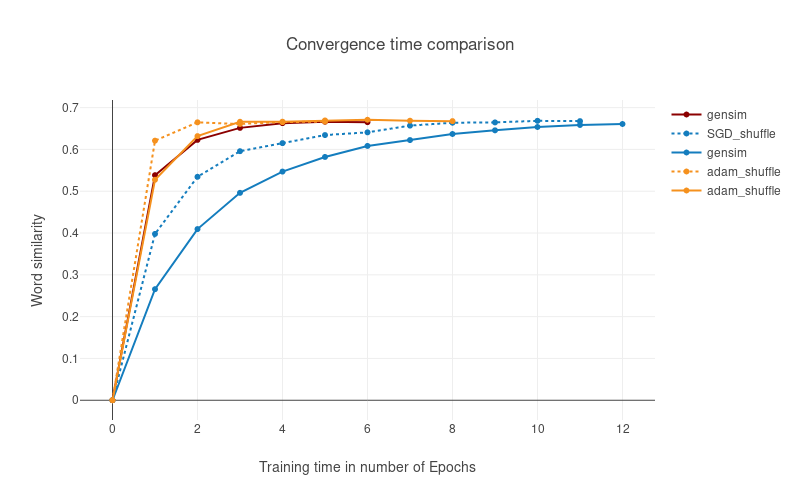
\includegraphics[scale=0.45]{images/gensim_vs_adam} 
    \caption{Training time Stochastic Gradient Descent with input Shuffling}
    \label{fig:gensim_vs_adam}
\end{figure}


\section{Further Work}
This work only focused on testing the approach of using advanced optimizers and input shuffling to improve the convergence time of the SGNS. While we did show that in theory it could work there still needs a bit of work to be done to show that this claim holds consistently.First and foremost an aspect of our implementation that can be prejudicial is that we only extensively tested our model with one small dataset. Both of these aspects are problematic. By using a very small dataset we do not use the model in the condition it is mostly needed for as the dataset used in practice a usually 3b words. There is a small argument that can be made for machine translation as the use of small parllel corpus is not unusual . But the main issue with using only one data set it that it has been shown that some optimizers perfrom better with specif shapes of loss functions. Hence it's necessary to show that Adam also outperfrom gensim with other data sets, to make a compelling argument. 
Furthermore having a better convergence time is not very useful if the runtime is hindered by a too complex computation, as for example second order optimization techniques. Therefore there is still need to show that Adam does not hinder computation time.  One would have to improve one of the already efficient implementation in order to show that we can imporve the convergence time while at the same time maintaining the same convergence time.



\section{Challenges faced}
During our implentation we did make some mistakes, this section has the purpose of informing the scientific community to not make the same mistakes. 
\subsection{Using the wrong embeddings}
To start with, we did not chose the same initialization value as gensim in our word embeddings. We initialized the input layer with a normal distribution between (-1,1). We did this because as we first started, we did indeed do the same thing as gensim, initializing the input layer with 0. But then our model did not seem to train well. Retrospectively we accord this to a learning rate too low. But back  then we changed the input layer intitialization. After a few trainings we saw that we did not perform as good as gensim. And as we changed theim back to 0 we performed well again. Therefore this is a recommendation to future work to not set the initialization to (-1,1).

\subsection{Batch size and loss function adjustements}\label{ssec:bs_lf}
During our experiments we faced a moment where we needed to us a very high learning rate (50) to achieve good results. As this is the complete opposite of what is standard we got suspiscous. To remedy the problem we made to changes. 
Firs we needed to find a good batch size. During the rise of the above training we used a batch size of 5000. We then decided to take a batch size of 2000.\\
 Secondly, at the same time we did experiment with different loss functions. As our batched model does not have exactly the same loss function as introduced by Mikolov et al. \cite{mikolov}. At the beginning of our experiment we took the average of all the scores stored in our final matrix. But then chose to take the sum as the training did not seem optimal.\\ 
 With these two changes we did increase convergence time and word similarity, and while at the same time having a usual learning rate. \\
 Know the question arises why this happened? Is this because the shape of the loss function better suits our advanced optimizers. Or because the loss function is closer to it's original form?

